\chapter{Programming with Pluto}
\label{cap4}

We already said our goal is to perform user-defined sensing tasks using nano-drones, in an indoor context.
We chose the Team Level approach, which we described in Section ~\ref{teamlevel}, applying some modifications to it, to manage the sensing tasks execution.
As we have shown in Section~\ref{teamlevelproblems}, the Team-Level approach is the most suitable approach for the kind of applications that can be developed with our framework.
The most important advantage of this approach is the reduced complexity given to the final user, while expressing the sensing tasks.
There is no need to describe how the drones should execute them.
These details are chosen by the Ground Control Station whose duty is to assign the right drone to the related task and check that each drone takes its mission to the end with a successful status.
In this chapter we describe the whole programming model of our system as a solution for the problems shown in Chapter \ref{cap3}.


\section{Programming model}\label{programmingModel}

Through our programming model, the user is able to specify a list of sensing tasks that the drones can perform.\\
Each one of the sensing tasks is represented by the \textit{Trip} entity, that is the virtual representation of a physical movement of the drone from a source location to a destination.
The Trip always ends with an \textit{Action}, that is the physical representation of the task. 
For example the drone can bring an \textit{Item}, take a photo or measure the temperature in a specific location.

Then, we decided to create a container entity called \textit{Mission}, that includes the list of tasks that the drones have to perform. 
This means that each Mission contains a list of trips.

It is important to underline that, inside each Mission entity, the trips are executed sequentially, one by one. 
The Mission entities, instead, are executed in parallel.
\\

So, to summarize, we identified the following entities:

\begin{itemize}
\itemsep2pt
\item{
\textbf{Mission}: a list of trips (sensing tasks) to be performed sequentially.
}
\item{
\textbf{Trip}: a Drone movement from a point A to a point B to perform an Action.
}
\item{
\textbf{Drone}: the physical executor of the Trip and the Action.
}
\item{
\textbf{Action}: the type of task to be performed by the Drone: "Take Photo", "Pick Item", "Release Item", "Measure", etc.
}
\item{
\textbf{Item}: the entity that represents the object carried by the Drone, only used in case of "Pick Item" and "Release Item" Actions.
}
\end{itemize}

\begin{figure}[htb]
  \centering
  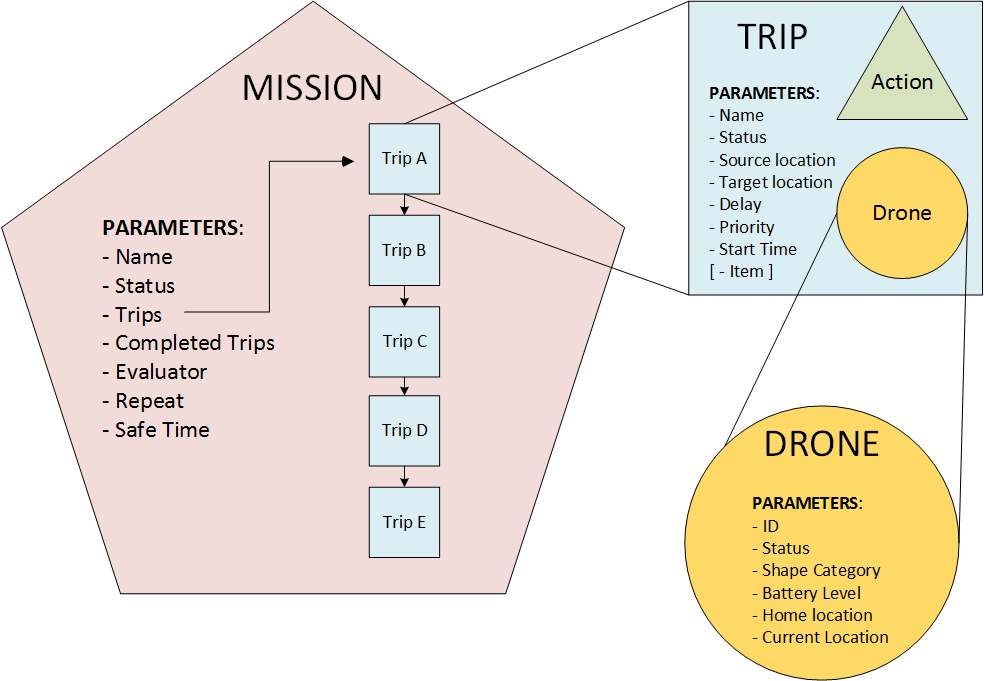
\includegraphics[width=\linewidth]
  {pictures/EntityRelationship.png}
  \caption{Relationship among model entities}
  \label{fig:EntityRelationship}
\end{figure}

\newpage

\underline{Mission}
\\

As shown in figure \ref{fig:EntityRelationship}, the Mission entity, in addition to the set of Trips, contains other important attributes that describe the Mission itself:

\begin{itemize}
\item{\textbf{Name}: the name given by the user while creating the mission}
\item{\textbf{Status}: describes how the Mission is being executed. For example, it is set to "RUNNING" while the drone is carrying out a Trip and to "FAILED" when a Trip fails because of a crash of the related Drone}
\item{\textbf{Trips}: the list of trips to be executed sequentially}
\item{\textbf{Completed Trips}: the trips completed successfully}
\item{\textbf{Evaluator}: the reference to the Evaluator entity. It is optional, and at the end of this Section we give a brief description of it}
\item{\textbf{Repeat}: states if the Mission must be repeated after its completion. It is optional, and we explain it in the MissionRepeater description in Section \ref{functionalBlocks}}
\item{\textbf{Safe Time}: contains the maximum amount of time within each trip inside the Mission must be completed. It is optional, and we explain it in the TimerMonitor description in Section \ref{functionalBlocks}}
\end{itemize}

\underline{Trip}
\\

Regarding the Trip entity, it contains several parameters too and furthermore it contains the references to the Drone  and Action entities.

\begin{itemize}
\item{\textbf{Name}: the name that identifies the Trip}
\item{\textbf{Status}: describes how the Trip is being executed. For example, it is set to "EXECUTING" while the drone is carrying out the Trip and to "FAILED" when a crash happens to the drone that is executing this Trip}
\item{\textbf{Source Location}: the starting point of the movement represented by the Trip}
\item{\textbf{Target Location}: the target point of the movement represented by the trip}
\item{\textbf{Delay}: the amount of time that the Trip must wait before starting.  It is optional, and we explain it in the Clock description in Section \ref{functionalBlocks}}
\item{\textbf{Priority}: states the priority level of the Trip.  It is optional, and we explain it in the PriorityManager description in Section \ref{functionalBlocks}}
\item{\textbf{Start Time}: contains the timestamp of the moment in which the Drone assigned to this Trip starts the flight.}
\item{\textbf{Item}: the attribute representing the Item that the assigned Drone brings. It is optional, based on the Action entity.}
\item{\textbf{Action}: the Action reference that describe the task to accomplish after the target location is reached.}
\item{\textbf{Drone}: the Drone reference that represents the physical drone assigned to the Trip.}
\end{itemize}

\underline{Drone}
\\

Another important entity in the programming model is the Drone. It represents the physical drone that performs the assigned Trip. It has some important parameters:

\begin{itemize}
\item{\textbf{ID}: it is a unique ID to distinguish each Drone}
\item{\textbf{Status}: states if the Drone is "FREE" and available for a trip or if it is "BUSY" because it is flying.}
\item{\textbf{Shape Category}: this parameter lets the system know if a drone is able to accomplish certain Action or move certain kind of Items.}
\item{\textbf{Battery Level}: contains the battery level of the Drone.}
\item{\textbf{Home Location}: contains the coordinates of the home location.}
\item{\textbf{Current Location}: contains the coordinates of the current location of the Drone. The system uses this parameter to localize the drone, when needed.}
\end{itemize}

\underline{Action}
\\

The Action entity describes the tasks that the drones must perform at the end of their trips.
We decided to create four basic actions whose names explain themselves: "Measure", "Take photo", "Pick item" and "Release Item". 
Moreover we added a "Custom Action" feature, which enables the developer to define a personal implementation of a new Action depending on the application requisites.
The developer can add this implementation after the code generation phase, explained in Section \ref{codeGeneration}, by adding his custom algorithm directly in the code.
\\

\underline{Evaluator}
\\

In figure \ref{fig:EntityRelationship}, inside the Mission object, there is a reference to the Evaluator entity. 
The Evaluator is the entity whose duty is to evaluate the outcomes of the actions performed inside a Mission.
\\
This means that some trips can be completed successfully but the Action done at the end can return a bad result. Therefore these actions should be repeated and so the related trips. 
This feature is provided by the MissionEvaluator functional block, described in Section \ref{functionalBlocks}.
\\
We decided to decouple this mechanism from our system, so that the developer is able to include its personal implementation of the evaluation algorithm in our framework. 
In Section \ref{codeGeneration} we describe this process in a more detailed way.
\\

\section{Functional blocks}
\label{functionalBlocks}

As already said in Section \ref{teamlevelproblems}, we decided to create a new dataflow programming framework that allows the user to design the behavior of the application while taking care of the missions execution.
\\

This framework consists of a modeling tool that allows the developer to add the application's requested features by drawing the proper nodes in an editor area.
\\
Each diagram created with this tool is made up of many functional blocks, each one including a particular logic.
The user can select the blocks needed for his particular application and connect them through simple connection elements.
The graphical editor is fully described in Section \ref{plutoGraphicalEditor}.
\\

Here we provide a detailed description of each functional block available in the editor:
\\

\underline{Mission Creator block}
\\

Input: a list of Trips

Output: a Mission object
\\

The Mission Creator block receives as an input the trips that the user wants to be performed by the drones, then it creates a Mission container including all these trips and returns that new Mission object.
This block is the starting point of each Pluto-developed application because it creates the Mission object that passes through all the blocks of the graph.
\\

\underline{Clock block}
\\

Input: a Mission object

Output: a Mission object
\\

The Clock block checks the delay attribute (Figure \ref{fig:EntityRelationship}) of the next Trip to be executed in the Mission. If it is greater than zero, it makes the Trip waiting for that amount of time, and finally returns the Mission Object.
Delaying the execution of the next Trip means stopping the Mission execution too, because, as said in Section \ref{programmingModel}, the trips are executed sequentially.
\\
If the programmer puts the Clock block in the graph, the Main Application will ask the user, during the Mission definition phase, the amount of time of the delay.
\\
This block can be used in an application where the user wants to measure the temperature in a location every 10 minutes.
He has to set a delay of 10 minutes for every Trip, so that they wait for that time before starting.
\\
Usually, this block is put between the Mission Creator and the Drone Allocator blocks, in order to wait for the delay time before allocating a Drone to the Trip.

\newpage

\underline{Drone Allocator block}
\\

Input: a Mission object

Output: a Mission object
\\

The Drone Allocator block allocates the proper Drone to the next Trip of the Mission taken as input.
It bases its choice on the availability of the drones and their capability to perform the desired action.
\\
This block can be implemented with different policies. Indeed, this choice is nothing but an optimization problem and the developer can choose a custom algorithm. 
We intentionally decoupled this problem from the system implementation, in a way that it is possible for the developer to change the policy as he wishes.
\\
This block is usually put before the Trip Launcher, because an assigned Drone is essential for the Trip execution.
For example it can be put between the Clock and the Trip Launcher blocks in order to assign a Drone to the next Trip,  after the delay time has passed.
\\

\underline{Trip Launcher block}
\\

Input: a Mission object

Output: a Mission object
\\

The Trip Launcher block takes the next Trip to be performed from the Mission, checks if it has an allocated Drone and then starts its execution.
The assigned Drone fly to the target location and execute the defined Action.
Usually this block is put right after the Drone Allocator, and is fundamental in order to start the execution of the trips of the Mission.
\\

\underline{Trip Monitor block}
\\

Input: a Mission object

Output: a Mission object
\\

The Trip Monitor block continuously checks the status of the Trip that is running in that moment.
As said in Section \ref{programmingModel}, the system executes the trips sequentially, so only one Trip at a time is executing and is monitored by this block. 
\\
We need to monitor the running trips because a flying Drone could crash or its battery could become empty before the end of the Trip. 
In this way we guarantee the correct completion of the Mission even if a failure happens.
\\
Depending on whether the Trip is failed or completed, this block changes its status parameter in the appropriate way.
Of course, the Mission that contains that Trip will change its status,accordingly.
The Trip Monitor is put after the Trip Launcher because it needs to monitor a Trip that already started its execution.
\\

\underline{Mission Repeater block}
\\

Input: a Mission object

Output: a Mission object
\\

This block takes as input only a completed Mission object.
\\
So when a completed Mission arrive to the Mission Repeater, the block verifies if the \textit{Repeat} attribute (Figure \ref{fig:EntityRelationship}) of the Mission is true.
if so, this block moves the list of the completed trips into the list of trips to be executed.
Then resets the status of the Mission itself and the status of all the trips to execute again.
\\
This block can be useful if a Mission has to be repeated many times.
For example, in a surveillance application, it lets the drones monitor the neighborhood without stopping when the Mission ends.
\\
In order to emulate this behavior without the block, the user should create a new identical Mission every time the previous one ends.
\\
This block is usually put after the Trip Monitor and before the Drone Allocator, because a Mission can be completed only after it pass through the Trip Monitor and the trips' status must be set to "WAITING" before the allocation of the drones.
\\

\underline{Mission Evaluator block}
\\

Input: a Mission object

Output: a Mission object
\\

The Mission Evaluator block, as the Mission Repeater, takes as input only a completed Mission.
Its task is to evaluate all the actions performed by the drones at the end of their trips.
Since the Mission arrives to this block only at the end of its lifecycle, all the trips are already executed and all the actions are already performed.
\\
The evaluation consists in invoking the \textit{Evaluator} entity, which is referenced inside the Mission object (Figure \ref{fig:EntityRelationship}).
\\
If the evaluation returns a fail result, it means that some actions should be repeated and the related trips too. 
The block finds these trips and put them in the list of trips to execute.
After that, it changes the status of the Mission, because it is not completed anymore since it has still some trips to complete.
\\
This block can be used in an application that needs to take many pictures of a natural site to build a map.
Therefore, the actions consist in taking photos at different coordinates and the evaluation in trying to build the whole map of the site stitching these photos together.
If some photos are not good enough, the evaluation returns a fail result and the related trips and actions are repeated again.
\\
Usually this block is put after the Trip Monitor and before the Drone Allocator for the same reasons explained in the description of the Mission Repeater block.
\\

\underline{Mission Modifier block}\label{missionModifier}
\\

Input: a Mission object

Output: a Mission object
\\

The Mission Modifier block allows the programmer to express new features, not yet implemented  by the existing functional blocks.
It allows the developer to create a brand new block performing a specific feature.
\\
This feature must be expressed with a code snippet that the developer can write directly in the editor.
\\
For example, imagine a programmer that needs a new feature that change some parameters of the Mission after the assignment of the Drone, but before the first Trip starts. 
He can insert the Mission Modifier block between the Drone Allocator and the Trip Launcher blocks. 
Then he can open the window shown in figure \ref{fig:missionmodifier} by clicking on the proper menu entry called "Write Custom Code".
\\
Inside this window, the programmer can write the code that describes the features requested by the new functional block.
So, following the example, here he changes the parameters of the Mission.
\\
In the end, we strongly recommend to rename the Mission Modifier block with a meaningful name that describes the new implemented  feature.
\\
This block can be put in every point of the Pluto Editor graph, depending on the particular feature it provides.
The inserted code is executed by the system when the Mission object reach this block, following the graph flow.
\\

\begin{figure}[H]
\centering
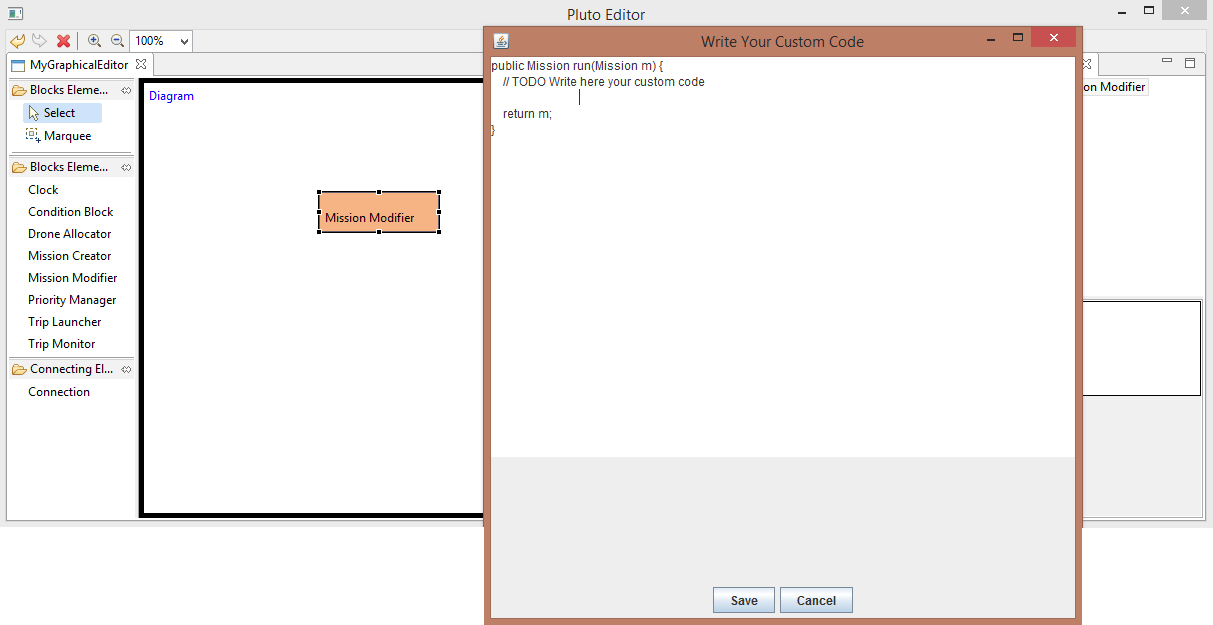
\includegraphics[width=\linewidth]
{pictures/MissionModifier.png}
  \caption{The MissionModifier block}
  \label{fig:missionmodifier}
\end{figure}

\newpage

\underline{PriorityManager block}
\\

Input: a Mission object

Output: a Mission object
\\

This block accepts as input only failed missions.
It takes the first Trip in the list and increments its priority.
After that, it sends the same Mission object as an output to the next blocks.
\\
This block is useful in order to not stop the execution flow of a Mission in case a Trip fails.
Normally, without this feature, if the Trip Monitor finds out that the monitored Trip has failed, it sets the Mission's status to FAILED and stops the execution flow.
\\
Instead this block raises the priority of the failed Trip and changes the status of the Mission to STANDBY, as if the failure is never happened.
\\
Then, to restart the execution flow of the Mission, we need a connection from the Priority Manager to the Drone Allocator.
\\

\underline{Timer Monitor block}
\\

Input: a Mission object

Output: a Mission object
\\

The Timer Monitor block adds a time constraint check to the Trip Monitor supervision. 
It is useless to add the Timer Monitor without the Trip Monitor, indeed they should be used in parallel.
\\
This means that while the Trip Monitor monitors the Trip execution, the Timer Monitor supervises the same Trip, ensuring that the execution time will not exceed the amount of time set in the "Safe Time" Mission's parameter (Figure \ref{fig:EntityRelationship}).
\\
As for the Trip Monitor, the developer should put the Timer Monitor after the Trip Launcher.
Therefore the Trip Launcher has two output connections, one that goes to the Trip Monitor and the other one that goes to the Timer Monitor.
\\
Adding this block in parallel to the Trip Monitor means cloning the Mission object which goes into the two blocks at the same time.
This is why we need the Gate blocks described further.
\\
There are several applications that could request the feature introduced by the Timer Monitor. 
Indeed it can be used to consider a Trip failed if its execution exceeds the Safe Time amount.
For example we could consider a drone crashed if the Trip takes more than 5 minutes to complete.
\\

\underline{Gate FIFO block}
\\

Input: a Mission object

Output: a Mission object
\\

The GateFIFO block is used when two or more blocks works in parallel, and only one instance of the Mission entity must propagate.
This block is put right after these parallel blocks, for example when the developer inserts in the graph either the Trip Monitor and the Timer Monitor in parallel. 
In this case the Mission object is cloned and the two blocks receive the same Mission object. 
The GateFIFO block propagates only the first Mission instance that arrives to it.
\\
The GateFIFO usually has more than one incoming connections and it propagates only the first Mission object arriving from them.
This is why the FIFO acronym is used, since the first Mission instance that arrive is the only one that propagates in the graph.
\\

\underline{Gate Funnel block}
\\

Input: a Mission object

Output: a Mission object
\\

This block is similar to the GateFIFO, but its implementation logic is different.
It waits for the Mission instances coming from each incoming connection.
Only after all of them arrive it merges them in one single instance and propagates it.
For example, if before this block, there are 4 blocks in parallel, the propagation of the Mission is activated only when all the 4 instances arrive.
\\

In figure \ref{fig:BlocksDiagram} we show an example application, which contains most of the blocks described above.
The pentagons represent the Mission object and the different colors stand for the status of the Mission while passing through the graph.
For example, after the Mission Creator every Mission's status is set to UNEXECUTED.
The Start and End blocks do not contain any logic, they simply represent the beginning and the end of the Mission flow.
\\

\begin{figure}[htb]
  \centering
  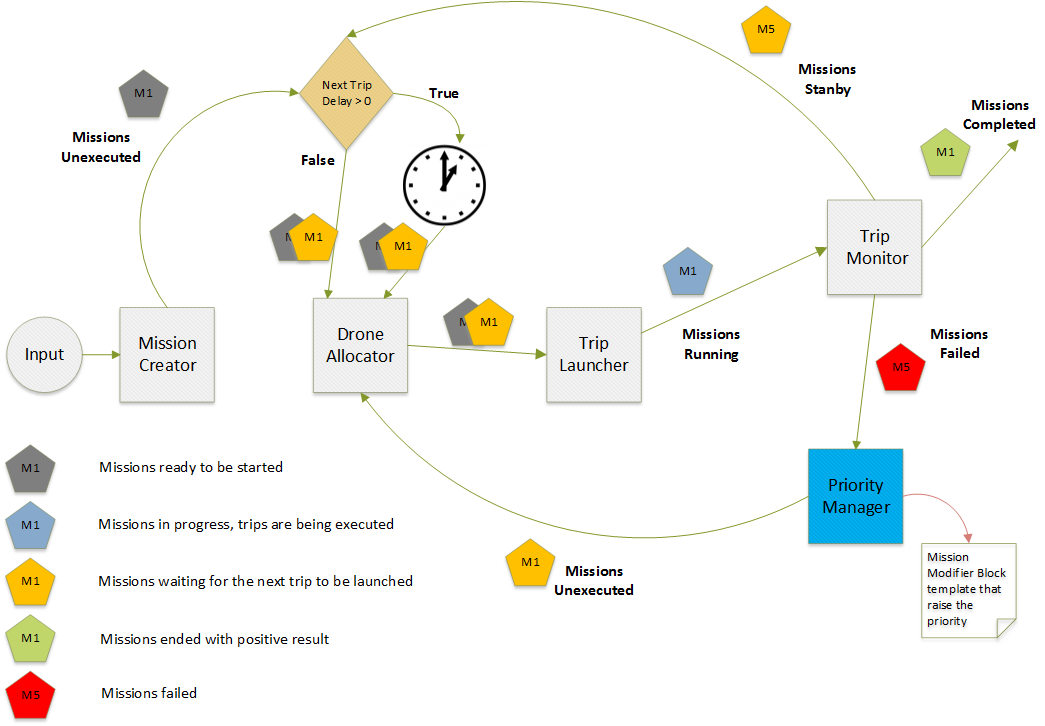
\includegraphics[width=\linewidth]{pictures/BlocksDiagram.png}
  \caption{An example Pluto application}
  \label{fig:BlocksDiagram}
\end{figure}

\section{Toolchain}\label{toolchain}

The Pluto programming framework consists of two main components:
\begin{itemize}
\item Pluto Graphical Editor.
\item Pluto Main Application.
\end{itemize}
The former is used by the first actor of the Pluto life-cycle: a developer. The latter is used by a final user whose duty is to insert the sensing tasks and to start their execution.
As shown in figure \ref{fig:lifeCycle}, the Pluto Graphical Editor lets the developer create a scenario based on the Team Level approach, as we show in Section ~\ref{plutoGraphicalEditor}.
After that, the Pluto Main Application is generated according to the diagram created in the previous step. 
The developer can create new features adding his own code, so that the final user needs only to insert the sensing tasks and wait for their accomplishment.

\begin{figure}[htb]
  \centering
  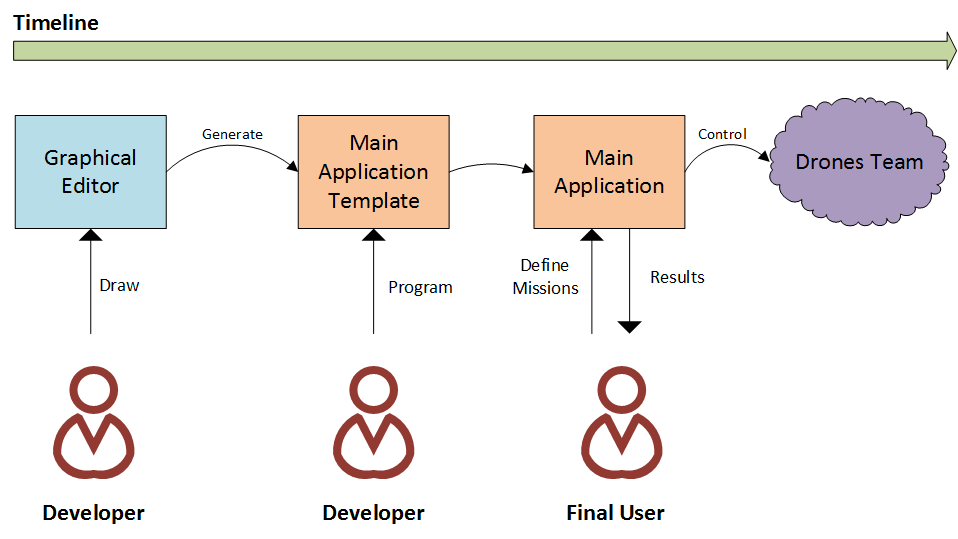
\includegraphics[width=\linewidth]{pictures/lifeCycle.png}
  \caption{Working with the Pluto framework}
  \label{fig:lifeCycle}
\end{figure}

\subsection{Pluto Graphical Editor}
\label{plutoGraphicalEditor}

We created a Graphical Editor in order to help the developer while designing the final application.
The provided tools can be used to link together different functional blocks, each one with a predefined and implemented logic.
When the Editor starts, it shows three main sections: 
the Palette (letter A in figure \ref{fig:GraphicalEditor}) that contains all the tools available to create a fully functional diagram.
The Editor space (letter B in figure \ref{fig:GraphicalEditor}) where the user can move, link and manage all the created entities.
Last but not least is the Outline (letter C in figure \ref{fig:GraphicalEditor}) with a tree-view of the blocks created by the developer in the editor space.

\begin{figure}[htb]
  \centering
  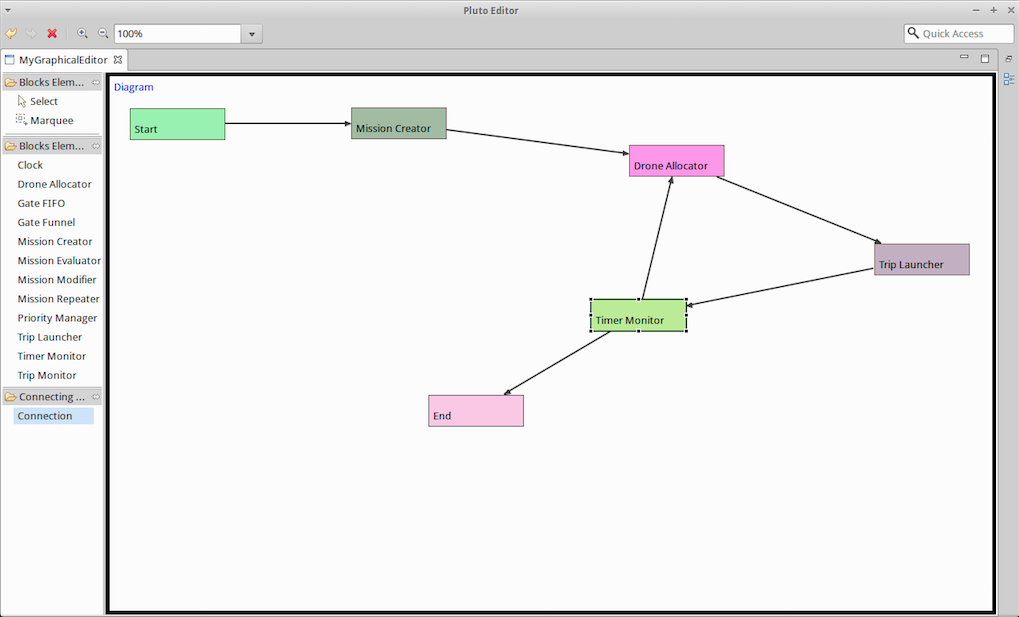
\includegraphics[width=\linewidth]{pictures/EditorScreen.png}
  \caption{Pluto Graphical Editor interface}
  \label{fig:GraphicalEditor}
\end{figure}

The developer can choose among several types of pre-created blocks, each one containing a certain logic, as explained in section \ref{functionalBlocks}. 
\\
Creating a block in the editor space can be done simply with a drag and drop gesture or clicking on the desired entity and then clicking on the chosen location in the editor. Then the user can connect the blocks using the Connection tool in the Palette section.
\\
The Connection is a directed arch that defines the direction of the execution flow in the graph. This means that the Mission entity traveling among the functional blocks can only move in the direction pointed out by the arrow.
\\
 
Apart from the standard functionality, such as Undo, Save, and Load, the Context Menu provides a command to generate the source-code of the Main Application, based on the designed diagram. The Toolbar provides Undo/Redo, Delete, and Magnify commands (letter D in in figure \ref{fig:GraphicalEditor}).
\\

To better understand the Pluto Graphical Editor, it is worth to clarify the meaning of creating a diagram:
each block in the diagram is a black box which is intended to manage a Mission entity. 
It takes a Mission as an input, works with it and sends it out as an output.
The connections among blocks represents the path that the Mission entity follows in the graph.
Each block can have multiple outgoing and incoming connections.
\\

In the editor area the developer creates a set of blocks linked together with a set of connections. This drawing can be interpreted as the behavior of the Main Application while managing the missions.
For example, figure \ref{fig:GraphicalEditor} represents the diagram that can handle the example described in Section \ref{motivating}.
\\
In this case the graph includes only the basic features: the creation of the Mission, the Drone assignation, the trips starting and their monitoring. 
It is possible to add other blocks in order to put more features in the application.
\\

Besides its simplicity our editor is very flexible, since it provides the Mission Modifier block whose implementation logic can be written directly in the Editor, by right-clicking on the block and choosing the option "Write Custom Code", as explained in Section \ref{functionalBlocks}.

\subsection{Pluto Main Application}
\label{plutoMainApp}

The Pluto Main Application is the final application that acts as a Ground Control Station, managing all the drones and the missions.
In this Section we explain how it works and how it can be used.
\\
Everything starts in the Mission Page where the user can define the tasks that will be carried out by the drones. After clicking to the "Add Mission" button the user is asked to set a name for the Mission.

\begin{figure}[H]
  \centering
  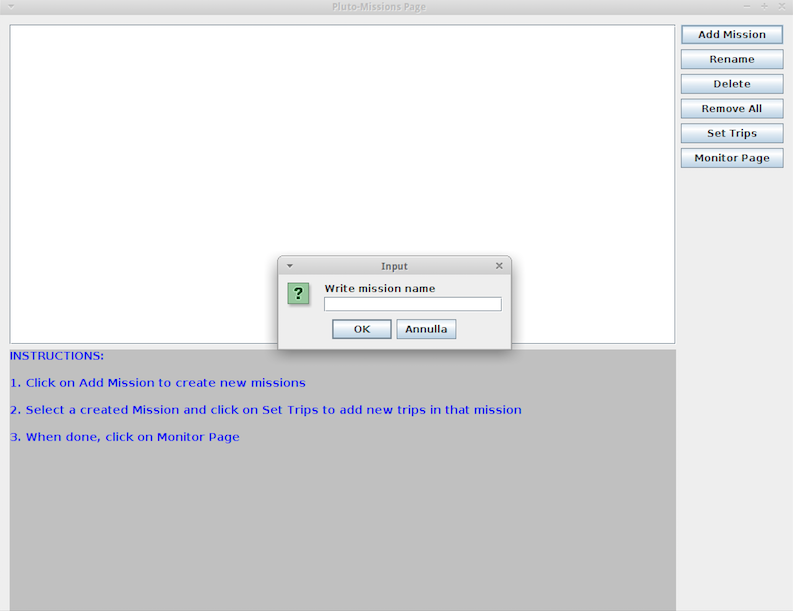
\includegraphics[width=\linewidth]{pictures/MissionPage.png}
  \caption{Mission Page interface}
  \label{fig:MissionPage}
\end{figure}

After that a Mission entity is created, but it does not contain any information about the tasks to execute. 
To add this information the user has to double-click on the mission in the main list, or click on the "Set Trips" button.
\\
A new window will appear, as shown in figure \ref{fig:TripsPage}, and the user can add new Trip entities to the related Mission.
As explained in Section \ref{programmingModel}, a Trip is nothing but a movement from point A to point B in the environment. 
The trips are the basic entities that constitute a single Mission. 
The single Trip contains information about the Action to execute once point B is reached.
\\
In order to add a new Trip the user can drag and drop the desired Action from the upper list (letter A in figure \ref{fig:TripsPage}) to the map displayed below (letter B in figure \ref{fig:TripsPage}).
The added trips are shown on the right, in a proper list (letter C in figure \ref{fig:TripsPage}).

\begin{figure}[H]
  \centering
  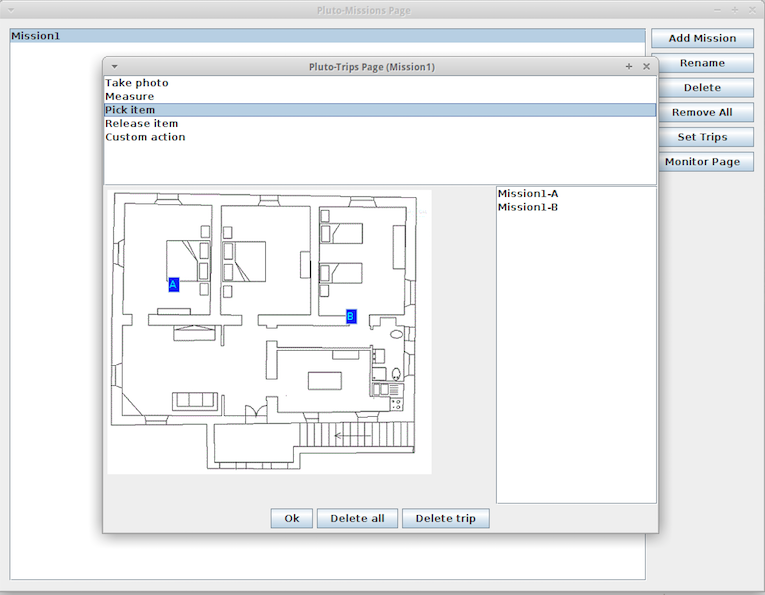
\includegraphics[width=\linewidth]{pictures/TripsPage.png}
  \caption{Trips Page interface}
  \label{fig:TripsPage}
\end{figure}

So, after all the Trips are added to the Mission, the user can close the Trips page and eventually create more Mission entities.
\\
Finally he can pass to the Monitor Page with the corresponding button.
The Monitor Page, shown in figure \ref{fig:MonitorPage}, is the window where the user can obtain information about the running missions, at run-time.
\\
On the top, there is a table (letter A in figure \ref{fig:MonitorPage}) where each row is assigned to a Mission.
Each column displays the information about the current Trip that is executing and the Drone assigned to that Trip.
\\
Below the table there is a console (letter B in figure \ref{fig:TripsPage}) where the log messages are printed during the execution of each mission.
In this way the user can obtain run-time information about the status of the entire system.
\\

Of course the "Start" button starts the execution of the created missions, while the "Stop" button brings the user to a make a choice: 
"RTL" or "Land".
The first is the Return To Launch and it makes all the drones return to the home location.
The second option makes all the drones land in their current locations. 
After the stop command, the missions status is preserved and the execution of the Mission can be started again in the future.

\begin{figure}[H]
  \centering
  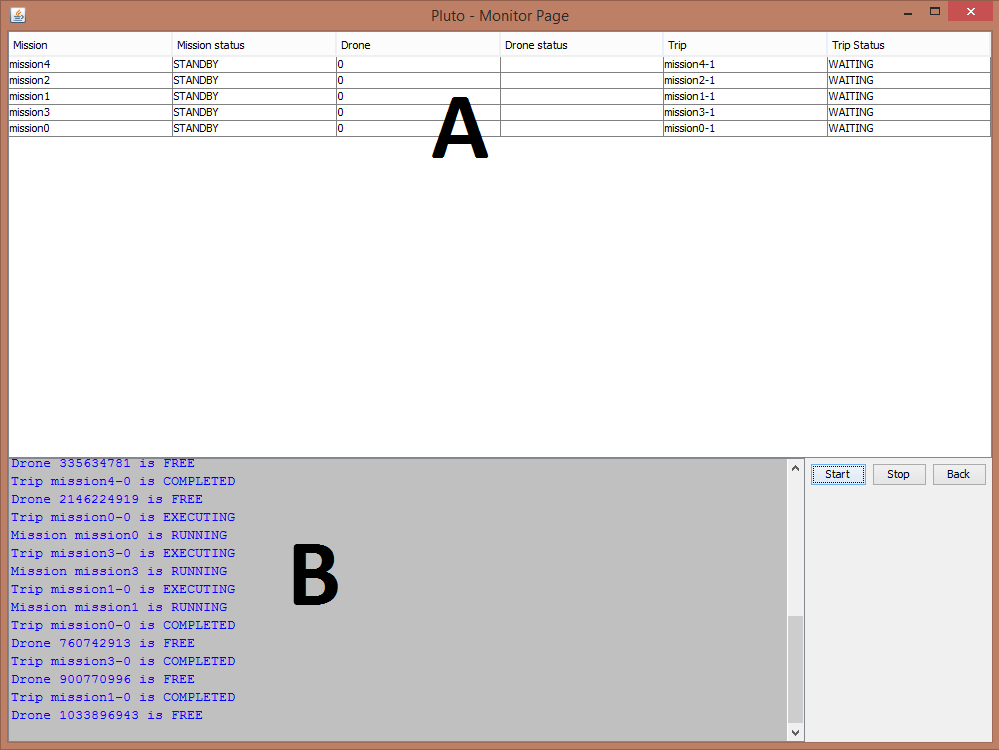
\includegraphics[width=\linewidth]{pictures/MonitorPage.png}
  \caption{Monitor Page interface}
  \label{fig:MonitorPage}
\end{figure}

\section{Navigation System}\label{navigationSystem}

An important component of the Main Application is the Navigation System.
More precisely, it is the conjunction point between the Main Application and the drones team. 

This component makes use of the chosen localization API to obtain precise coordinates for each Drone.
This API depends on the technologies chosen to localize the drones in the indoor context, described in Section \ref{indoor}.
\\ 

We decided to decouple the implementation of the Navigation System from the Main Application, so that the developer is free to choose the technology he prefers.
This result can be achieved by adding the chosen API in the Navigation System component, without modifying other parts of the Main Application.
\\
This choice derived from the conclusions obtained in Chapter \ref{cap3}, where we discussed about some possible ways to enable the indoor localization.
\\
The Navigation System, as said, is the internal component that directly communicates with the drones team. 
This means that besides the localization API, it makes also use of specific drone libraries.
In Section \ref{crazyflie} we give a brief description of the API of the drone we chose for our prototype applications, the Crazyflie nano-quadcopter.
\\

\section{Design Choices}\label{history}

In this section we describe our previously developed solutions, which we refined many times in order to obtain the final working version of the Pluto programming framework; this is done by using a top-down approach, starting from the final implementation to the very first one.

\subsection{Solution without Trip entity}

In the version precedent to the final solution presented in Section \ref{programmingModel}, we did not have a concept of Trip, and the Mission was the main concept the whole model was based on. 
Figure \ref{fig:noTrip} shows this in the particular case of the Timer feature, which contains also a "Switch source-target" block. 
This block was in charge to make the Drone perform also the return journey, from the destination to the home location.
This is done inside the same Trip entity, simply switching its \textit{sourceLocation} and \textit{targetLocation} attributes.
Later this block was eliminated, since we decided to decouple the two journeys.
It is sufficient to create a new Trip entity for the return journey.

\begin{figure}[H]
  \centering
  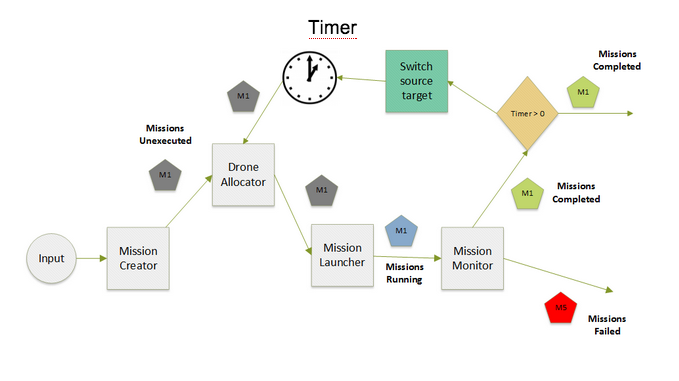
\includegraphics[width=\linewidth]{pictures/NoTrip.png}
  \caption{Solution without the Trip concept}
  \label{fig:noTrip}
\end{figure}

After analyzing the model, we realized that we needed the concept of Trip, because the final user must have control on the single Trip of a drone, in order to decide which action the drone must perform, and to have an opportunity to control the Trip attributes such as delay, stop, or delete, without deleting or stop the whole Mission. 
With this solution it was not possible, because having only the entire Mission to manage, the user cannot control the single Trip, and if he/she wants to delete only a part of the Mission he cannot do so, and he/she is forced to delete and build again the whole Mission.

\subsection{Solution without the DroneAllocator and MissionModifier}

This solution made use of the "Drone Updater" block instead of the DroneAllocator. 
This block managed the assignment of a Drone to a Mission(there was not the Trip concept yet), but only under certain conditions.
Indeed the "Drone Updater" was used only if the system had to assign another drone to a Mission, for example because of a failure of the precedent assigned Drone.
This happened because the MissionCreator managed the first assignment of a Drone to the Mission, so we did not need the DroneUpdater for the first assignment of a Drone to a Mission.
Furthermore, there was not the MissionModifier block, but only the PriorityManager case, shown in figure \ref{fig:noMM}, so the programmer could not insert his custom code in the application.


\begin{figure}[H]
  \centering
  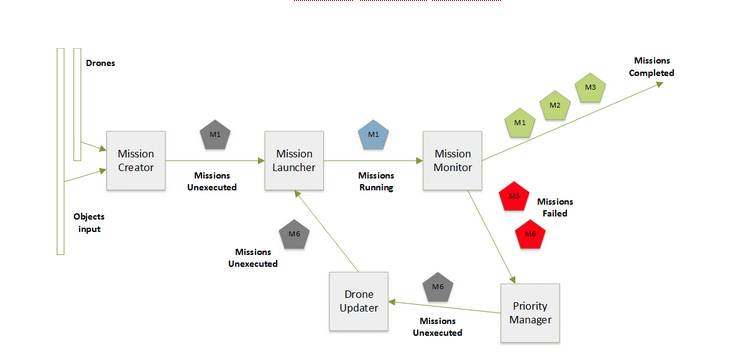
\includegraphics[width=\linewidth]{pictures/NoMM.png}
  \caption{Solution without the MissionModifier block}
  \label{fig:noMM}
\end{figure}

We decided to create the DroneAllocator block because we needed to separate the creation of a Mission Object from the assignment of a Drone to it.
So, the MissionCreator should only create a Mission entity and the DroneAllocator should take care of the drones dispatching.
In this way we could also remove the "Drone Updater" block, because now we have a specific block which manage only the assignment of drones, so there is no more need to distinguish between the first assignment of a Drone to a Mission and the "special assignment" in case of a failure.
We also decided to create a MissionModifier block in which the user can put his own code to customize the application.